% Options for packages loaded elsewhere
\PassOptionsToPackage{unicode}{hyperref}
\PassOptionsToPackage{hyphens}{url}
%
\documentclass[
]{article}
\usepackage{lmodern}
\usepackage{amssymb,amsmath}
\usepackage{ifxetex,ifluatex}
\ifnum 0\ifxetex 1\fi\ifluatex 1\fi=0 % if pdftex
  \usepackage[T1]{fontenc}
  \usepackage[utf8]{inputenc}
  \usepackage{textcomp} % provide euro and other symbols
\else % if luatex or xetex
  \usepackage{unicode-math}
  \defaultfontfeatures{Scale=MatchLowercase}
  \defaultfontfeatures[\rmfamily]{Ligatures=TeX,Scale=1}
\fi
% Use upquote if available, for straight quotes in verbatim environments
\IfFileExists{upquote.sty}{\usepackage{upquote}}{}
\IfFileExists{microtype.sty}{% use microtype if available
  \usepackage[]{microtype}
  \UseMicrotypeSet[protrusion]{basicmath} % disable protrusion for tt fonts
}{}
\makeatletter
\@ifundefined{KOMAClassName}{% if non-KOMA class
  \IfFileExists{parskip.sty}{%
    \usepackage{parskip}
  }{% else
    \setlength{\parindent}{0pt}
    \setlength{\parskip}{6pt plus 2pt minus 1pt}}
}{% if KOMA class
  \KOMAoptions{parskip=half}}
\makeatother
\usepackage{xcolor}
\IfFileExists{xurl.sty}{\usepackage{xurl}}{} % add URL line breaks if available
\IfFileExists{bookmark.sty}{\usepackage{bookmark}}{\usepackage{hyperref}}
\hypersetup{
  pdftitle={Assignment 9.2 - Intoduction to Machine Learning},
  pdfauthor={edris safari},
  hidelinks,
  pdfcreator={LaTeX via pandoc}}
\urlstyle{same} % disable monospaced font for URLs
\usepackage[margin=1in]{geometry}
\usepackage{graphicx,grffile}
\makeatletter
\def\maxwidth{\ifdim\Gin@nat@width>\linewidth\linewidth\else\Gin@nat@width\fi}
\def\maxheight{\ifdim\Gin@nat@height>\textheight\textheight\else\Gin@nat@height\fi}
\makeatother
% Scale images if necessary, so that they will not overflow the page
% margins by default, and it is still possible to overwrite the defaults
% using explicit options in \includegraphics[width, height, ...]{}
\setkeys{Gin}{width=\maxwidth,height=\maxheight,keepaspectratio}
% Set default figure placement to htbp
\makeatletter
\def\fps@figure{htbp}
\makeatother
\setlength{\emergencystretch}{3em} % prevent overfull lines
\providecommand{\tightlist}{%
  \setlength{\itemsep}{0pt}\setlength{\parskip}{0pt}}
\setcounter{secnumdepth}{-\maxdimen} % remove section numbering

\title{Assignment 9.2 - Intoduction to Machine Learning}
\author{edris safari}
\date{2/7/2020}

\begin{document}
\maketitle

\hypertarget{assignment-9.2---intoduction-to-machine-learning}{%
\subsection{Assignment 9.2 - Intoduction to Machine
Learning}\label{assignment-9.2---intoduction-to-machine-learning}}

Regression algorithms are used to predict numeric quantity while
classification algorithms predict categorical outcomes. A spam filter is
an example use case for a classification algorithm. The input dataset is
emails labeled as either spam (i.e.~junk emails) or ham (i.e.~good
emails). The classification algorithm uses features extracted from the
emails to learn which emails fall into which category.

In this problem, you will use the nearest neighbors algorithm to fit a
model on two simplified datasets. The first dataset (found in
\url{binary-classifier-data.csv} contains three variables; label, x, and
y. The label variable is either 0 or 1 and is the output we want to
predict using the x and y variables. The second dataset (found in
\url{trinary-classifier-data.csv} is similar to the first dataset except
for the label variable can be 0, 1, or 2.

Note that in real-world datasets, your labels are usually not numbers,
but text-based descriptions of the categories (e.g.~spam or ham). In
practice, you will encode categorical variables into numeric values.

\begin{enumerate}
\def\labelenumi{\alph{enumi}.}
\item
  Plot the data from each dataset using a scatter plot.
\item
  The k nearest neighbors algorithm categorizes an input value by
  looking at the labels for the k nearest points and assigning a
  category based on the most common label. In this problem, you will
  determine which points are nearest by calculating the Euclidean
  distance between two points. As a refresher, the Euclidean distance
  between two points: p1=(x1, y1) and p2=(x2,y2) is
  d=\(\sqrt{(x_1 - X_2)^2 + (y_1 - Y_2)^2}\).

  Fitting a model is when you use the input data to create a predictive
  model. There are various metrics you can use to determine how well
  your model fits the data. You will learn more about these metrics in
  later lessons. For this problem, you will focus on a single metric;
  accuracy. Accuracy is simply the percentage of how often the model
  predicts the correct result. If the model always predicts the correct
  result, it is 100\% accurate. If the model always predicts the
  incorrect result, it is 0\% accurate.

  Fit a k nearest neighbors model for each dataset for k=3, k=5, k=10,
  k=15, k=20, and k=25. Compute the accuracy of the resulting models for
  each value of k. Plot the results in a graph where the x-axis is the
  different values of k and the y-axis is the accuracy of the model.
\item
  In later lessons, you will learn about linear classifiers. These
  algorithms work by defining a decision boundary that separates the
  different categories.
\end{enumerate}

\begin{figure}
\centering
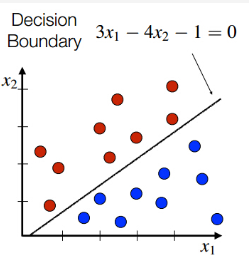
\includegraphics{DecisionBoundary.png}
\caption{Decision Boundary}
\end{figure}

Looking back at the plots of the data, do you think a linear classifier
would work well on these datasets?

\hypertarget{import-dataset}{%
\subsubsection{Import dataset}\label{import-dataset}}

\begin{verbatim}
## [1] "C:/Users/safar/Documents/GitHub/Safarie1103/Bellevue University/Courses/DSC520/Week9"
\end{verbatim}

\begin{verbatim}
## [1] "C:/Users/safar/Documents/GitHub/Safarie1103/Bellevue University/Courses/DSC520/Week9"
\end{verbatim}

\begin{verbatim}
##          x        y label
## 1 70.88469 83.17702     0
## 2 74.97176 87.92922     0
## 3 73.78333 92.20325     0
## 4 66.40747 81.10617     0
## 5 69.07399 84.53739     0
## 6 72.23616 86.38403     0
\end{verbatim}

\begin{verbatim}
##          x        y label
## 1 30.08387 39.63094     0
## 2 31.27613 51.77511     0
## 3 34.12138 49.27575     0
## 4 32.58222 41.23300     0
## 5 34.65069 45.47956     0
## 6 33.80513 44.24656     0
\end{verbatim}

\hypertarget{scatter-plots}{%
\subsubsection{Scatter plots}\label{scatter-plots}}

\hypertarget{scatter-plot-of-binary-data}{%
\paragraph{Scatter plot of binary
data}\label{scatter-plot-of-binary-data}}

\includegraphics{Assignment-9.2-IntroductionToMachineLearning_files/figure-latex/scatter plot binary-1.pdf}

\hypertarget{scatter-plot-of-trinary-data}{%
\paragraph{Scatter plot of trinary
data}\label{scatter-plot-of-trinary-data}}

\includegraphics{Assignment-9.2-IntroductionToMachineLearning_files/figure-latex/scatter plot trinary-1.pdf}

\begin{verbatim}
##          x        y label Clusters
## 1 70.88469 83.17702     0        4
## 2 74.97176 87.92922     0        4
## 3 73.78333 92.20325     0        4
## 4 66.40747 81.10617     0        4
## 5 69.07399 84.53739     0        4
## 6 72.23616 86.38403     0        4
\end{verbatim}

\begin{verbatim}
##          x        y label Clusters
## 1 30.08387 39.63094     0        5
## 2 31.27613 51.77511     0        3
## 3 34.12138 49.27575     0        3
## 4 32.58222 41.23300     0        5
## 5 34.65069 45.47956     0        3
## 6 33.80513 44.24656     0        3
\end{verbatim}

\includegraphics{Assignment-9.2-IntroductionToMachineLearning_files/figure-latex/3-1.pdf}
\includegraphics{Assignment-9.2-IntroductionToMachineLearning_files/figure-latex/4-1.pdf}

\begin{verbatim}
##           x        y label
## 2  74.97176 87.92922     0
## 4  66.40747 81.10617     0
## 5  69.07399 84.53739     0
## 8  77.57454 98.63425     0
## 11 67.20828 85.62172     0
## 16 69.23680 89.98705     0
\end{verbatim}

\begin{verbatim}
## [1] 0 0 0 0 0 0
## Levels: 0 1
\end{verbatim}

\begin{verbatim}
##    y_pred
##       0   1
##   0 186   6
##   1   4 179
\end{verbatim}

\includegraphics{Assignment-9.2-IntroductionToMachineLearning_files/figure-latex/Visualising the Training set results -1.pdf}

\includegraphics{Assignment-9.2-IntroductionToMachineLearning_files/figure-latex/unnamed-chunk-2-1.pdf}

\end{document}
